\section{Traditional Approach} 
Real-life ear images can be acquired in various formats with different scaling and rota- tion conditions. In this paper, we propose to use scale and rotation invariant feature detectors to describe interested features and match them with other images in the data- bases. The proposed ear recognition technique is shown in Figure 1.1. Below is a brief description of each function block.


\begin{figure}
\centering
\begin{subfigure}{.5\textwidth}
  \centering
  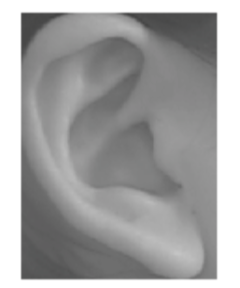
\includegraphics[width=.4\linewidth]{Figures/Figure3}
  \caption{Original Ear Image}
  \label{fig:sub1}
\end{subfigure}%
\begin{subfigure}{.5\textwidth}
  \centering
  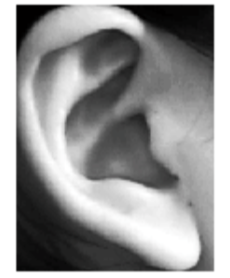
\includegraphics[width=.4\linewidth]{Figures/Figure4}
  \caption{Enhanced Ear image}
  \label{fig:sub2}
\end{subfigure}
\caption{Ear Image Enhancement}
\label{fig:test}
\end{figure}

\begin{figure}
\centering
\begin{minipage}{.5\textwidth}
  \centering
  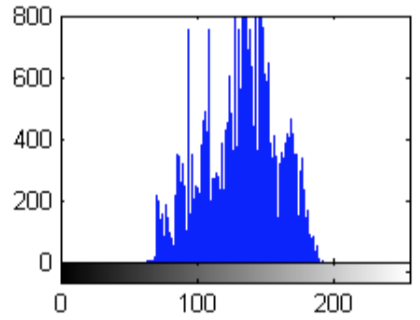
\includegraphics[width=.4\linewidth]{Figures/Figure5}
  \captionof{figure}{Histogram of Original Image}
  \label{fig:test1}
\end{minipage}%
\begin{minipage}{.5\textwidth}
  \centering
  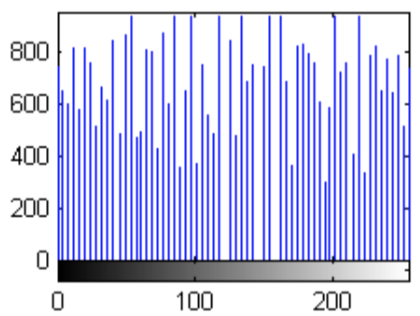
\includegraphics[width=.4\linewidth]{Figures/Figure6}
  \captionof{figure}{Histogram of Enhanced Image}
  \label{fig:test2}
\end{minipage}
\end{figure}



The ear enhancement process starts with contrast enhancement, where we apply histo- gram equalization to improve the contrast in an image in order to stretch out its intensity range, from which, we get an enhanced version of the original image by maximizing the contrast level of an image, as shown in


 table \ref{tab:commands1}.

\begin{table}
\caption{\label{tab:commands1}Command Set of Scheduler Module, Build 1}
\centering
\begin{tabular}{llp{3.0in}}
\hline
\multicolumn{1}{c}{\textbf{Type}} &
\multicolumn{1}{c}{\textbf{Name}} &
\multicolumn{1}{c}{\textbf{Actions}} \\
\hline
TMcom	&	Enqueue				& Schedules a thread\\
TMcom	&	Dequeue				& Removes a thread from the ready-to-run queue	\\
BUScom	&	Get\_Entry     		& Returns a thread's table attribute entry		\\
BUScom	&	Toggle\_Preemption	& Toggle preemption interrupt on/off	\\
BUScom	&	Get\_Entry     		& Returns a thread's table attribute entry (for debug use)		\\
BUScom	&	Get\_Priority		& Returns the priority-level of a thread	\\
BUScom	&	Set\_Priority		& Sets the priority-level of a thread\\
BUScom	&	Set\_Default\_Priority		& Sets the priority-level of a thread (no error-checking)\\
\hline
\end{tabular}
\end{table}

